\chapter{Data Application} \label{chapter4:Data-Application}

To evaluate the performance of our method on real data, we use an atomic force microscopy (AFM) image of a solar cell. The image (see Figure~\ref{fig:film}) comes from a paper by Singh et al.~\cite{Singh2014}, who wanted to improve efficiency of converting light into electricity by optimizing the concentration of carbon nanotubes in solar cells coated with a particular compound called poly(3-hexylthiophene): phenyl-C61-butyric acid methyl ester (P3HT:PCBM). This compound is spread in a microscopically thin film over the cell.

\begin{figure}[htbp]
	\centering
	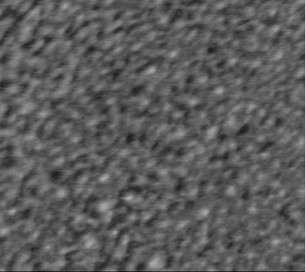
\includegraphics[width=0.65\textwidth]{film.png}
	\caption{Atomic force microscopy image of a thin film of the P3HT:PCBM compound on a solar cell. Dark clusters represent areas where the film is thinner, and lighter clusters are thicker areas.}
	\label{fig:film}
\end{figure}

Figure~\ref{fig:film} shows a P3HT:PCBM film doped with a 0.1\% concentration of carbon nanotubes. By treating the film thickness as observations from an unknown isotropic stationary Gaussian process, our goal was to train a covariance model on some of these observations and predict the others.

To prepare the data, we selected ten 25-by-25 pixel squares to use to estimate the covariance function. We treated the squares as 10 independent observations of a Gaussian process on the 25-by-25 grid. Once we obtained our estimate, we selected an out of sample 25-by-25 square, removed a 4-by-4 section of that square made predictions conditionally on the remainder as observations in the square. One of the training squares is shown in Figure~\ref{fig:training25}, and Figure~\ref{fig:pred25} shows the observation square, with the withheld prediction points highlighted in red.

\begin{figure}[htbp]
	\centering
	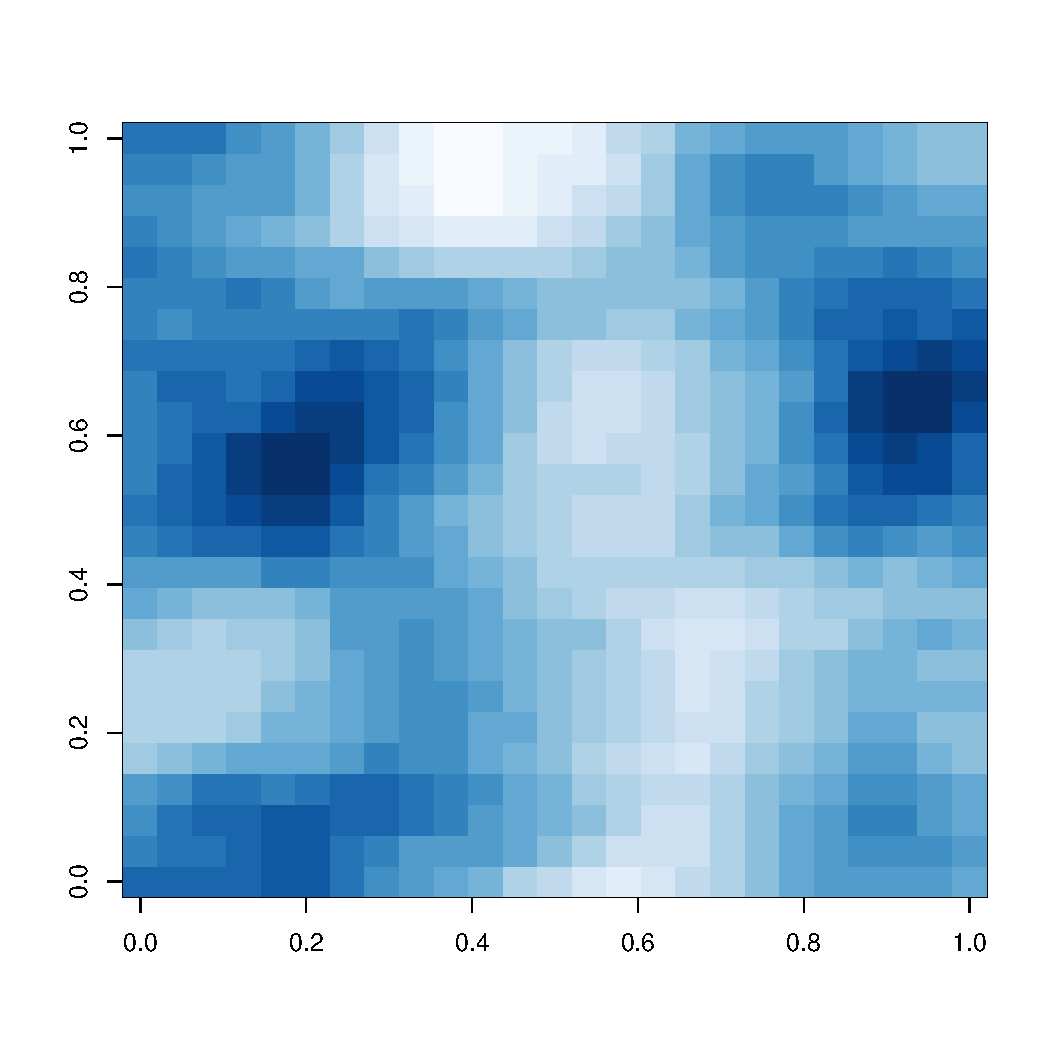
\includegraphics[width=0.95\textwidth]{col_image_5.pdf}
	\caption{One of the 10 25-by-25 sections of the film image used to fit the spline model.}
	\label{fig:training25}
\end{figure}

\begin{figure}[htbp]
	\centering
	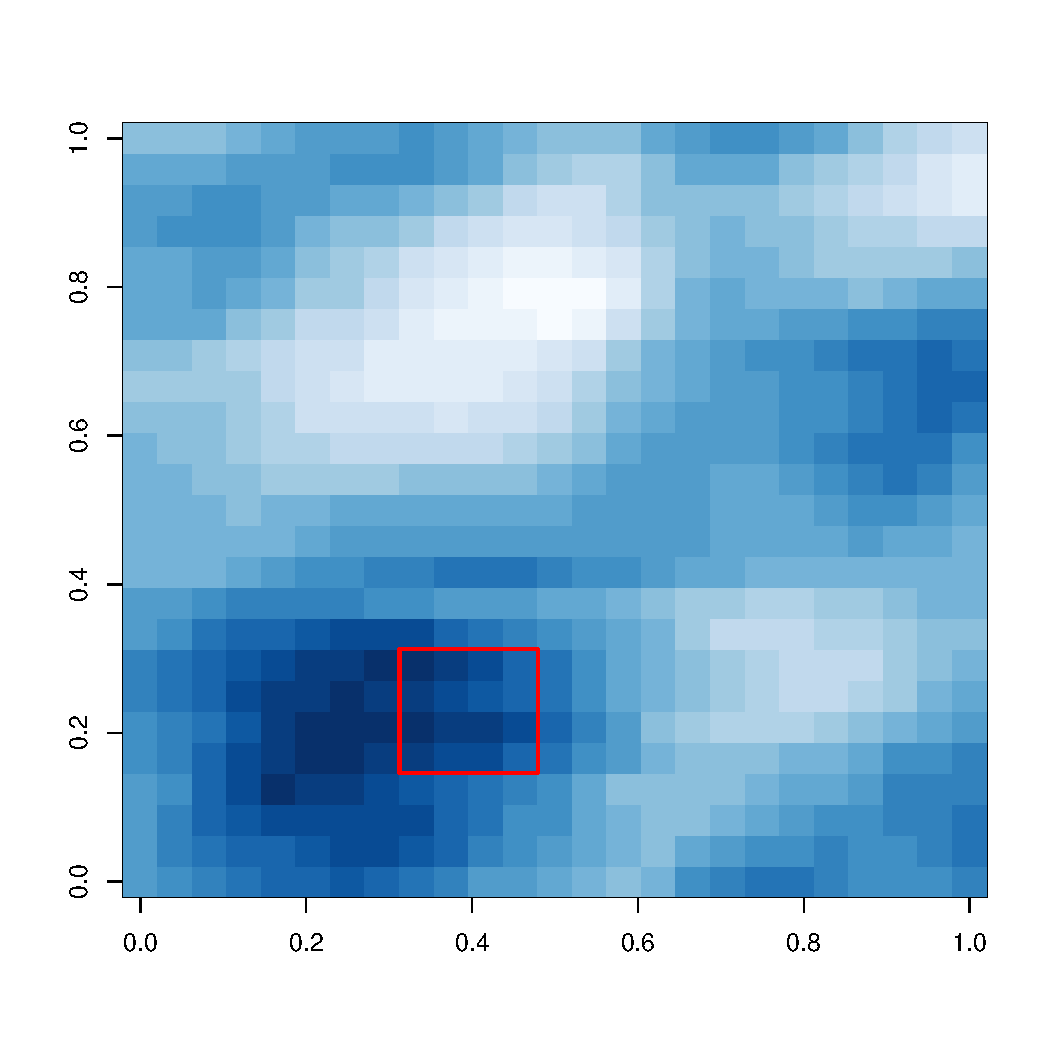
\includegraphics[width=0.95\textwidth]{col_pred.pdf}
	\caption{This 25-by-25 section of the film image was held out from the training step. The 16 outlined pixels are used for prediction, and the others are treated as observations.}
	\label{fig:pred25}
\end{figure}

\begin{figure}[htbp]
	\centering
	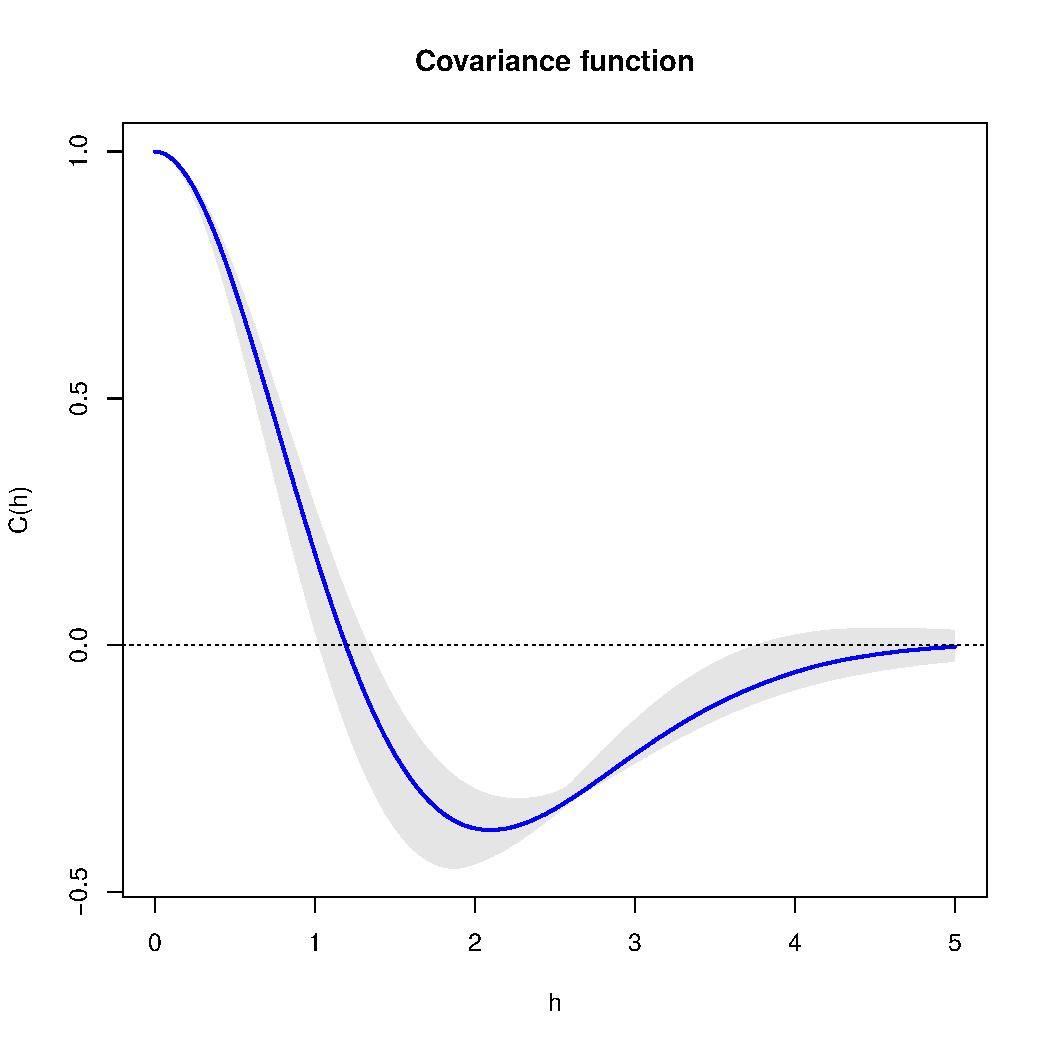
\includegraphics[width=0.95\textwidth]{covariance_realdata.pdf}
	\caption{The estimated covariance function based on the 10 25-by-25 sections of the film image used to fit the spline model.}
	\label{fig:covariance-realdata}
\end{figure}

We fit the semiparametric model and a Mat\'ern model, and compare the prediction performance of each. The mean squared prediction error for the Mat\'ern model was $0.0008707$, while the mean squared prediction error for the semiparametric model was $0.0006414$. The semiparametric model performed $26.3\%$ better on the 16 prediction points, indicating that it is capturing the local behavior of the Gaussian process more effectively than the best-fit Mat\'ern model can. Figure~\ref{fig:covariance-realdata} shows the estimated covariance function from the semiparametric model. There is a significant hole effect that a Mat\'ern model is not capable of capturing.
